\documentclass[a4paper, 14pt]{extarticle}
\usepackage[settings]{markdown}
\usepackage{minted}

% Поля
%--------------------------------------
\usepackage{geometry}
\geometry{a4paper,tmargin=2cm,bmargin=2cm,lmargin=3cm,rmargin=1cm}
%--------------------------------------


%Russian-specific packages
%--------------------------------------
\usepackage[T2A]{fontenc}
\usepackage[utf8]{inputenc} 
\usepackage[english, main=russian]{babel}
%--------------------------------------

\usepackage{textcomp}

% Красная строка
%--------------------------------------
\usepackage{indentfirst}               
%--------------------------------------             


%Graphics
%--------------------------------------
\usepackage{graphicx}
\graphicspath{ {./images/} }
\usepackage{wrapfig}
%--------------------------------------

% Полуторный интервал
%--------------------------------------
\linespread{1.3}                    
%--------------------------------------

%Выравнивание и переносы
%--------------------------------------
% Избавляемся от переполнений
\sloppy
% Запрещаем разрыв страницы после первой строки абзаца
\clubpenalty=10000
% Запрещаем разрыв страницы после последней строки абзаца
\widowpenalty=10000
%--------------------------------------

%Списки
\usepackage{enumitem}

%Подписи
\usepackage{caption} 

%Гиперссылки
\usepackage{hyperref}

\hypersetup {
	unicode=true
}

%Рисунки
%--------------------------------------
\DeclareCaptionLabelSeparator*{emdash}{~--- }
\captionsetup[figure]{labelsep=emdash,font=onehalfspacing,position=bottom}
%--------------------------------------

\usepackage{tempora}
\usepackage{amsmath}
\usepackage{color}
\usepackage{listings}
\lstset{
  belowcaptionskip=1\baselineskip,
  breaklines=true,
  frame=L,
  xleftmargin=\parindent,
  language=Python,
  showstringspaces=false,
  basicstyle=\footnotesize\ttfamily,
  keywordstyle=\bfseries\color{blue},
  commentstyle=\itshape\color{purple},
  identifierstyle=\color{black},
  stringstyle=\color{red},
}

%--------------------------------------
%			НАЧАЛО ДОКУМЕНТА
%--------------------------------------

\begin{document}

%--------------------------------------
%			ТИТУЛЬНЫЙ ЛИСТ
%--------------------------------------
\begin{titlepage}
\thispagestyle{empty}
\newpage


%Шапка титульного листа
%--------------------------------------
\vspace*{-60pt}
\hspace{-65pt}
\begin{minipage}{0.3\textwidth}
\hspace*{-20pt}\centering

\includegraphics[width=\textwidth]{emblem}
\end{minipage}
\begin{minipage}{0.67\textwidth}\small \textbf{
\vspace*{-0.7ex}
\hspace*{-6pt}\centerline{Министерство науки и высшего образования Российской Федерации}
\vspace*{-0.7ex}
\centerline{Федеральное государственное бюджетное образовательное учреждение }
\vspace*{-0.7ex}
\centerline{высшего образования}
\vspace*{-0.7ex}
\centerline{<<Московский государственный технический университет}
\vspace*{-0.7ex}
\centerline{имени Н.Э. Баумана}
\vspace*{-0.7ex}
\centerline{(национальный исследовательский университет)>>}
\vspace*{-0.7ex}
\centerline{(МГТУ им. Н.Э. Баумана)}}
\end{minipage}
%--------------------------------------

%Полосы
%--------------------------------------
\vspace{-25pt}
\hspace{-35pt}\rule{\textwidth}{2.3pt}

\vspace*{-20.3pt}
\hspace{-35pt}\rule{\textwidth}{0.4pt}
%--------------------------------------

\vspace{1.5ex}
\hspace{-35pt} \noindent \small ФАКУЛЬТЕТ\hspace{50pt} <<Информатика и системы управления>>

\vspace*{-16pt}
\hspace{47pt}\rule{0.83\textwidth}{0.4pt}

\vspace{0.5ex}
\hspace{-35pt} \noindent \small КАФЕДРА\hspace{50pt} <<Теоретическая информатика и компьютерные технологии>>

\vspace*{-16pt}
\hspace{30pt}\rule{0.866\textwidth}{0.4pt}
  
\vspace{11em}

\begin{center}
\Large {\bf Лабораторная работа № 4} \\ 
\large {\bf по курсу <<Распределение параллельных и распределённых программ>>}\\
\large <<Задача о пяти обедающих философах>>
\end{center}\normalsize

\vspace{8em}


\begin{flushright}
  {Студент группы ИУ9-51Б Горбунов А. Д.\hspace*{15pt} \\
  \vspace{2ex}
  Преподаватель Царёв А. С.\hspace*{15pt}}
\end{flushright}

\bigskip

\vfill
 

\begin{center}
\textsl{Москва 2024}
\end{center}
\end{titlepage}
%--------------------------------------
%		КОНЕЦ ТИТУЛЬНОГО ЛИСТА
%--------------------------------------

\renewcommand{\ttdefault}{pcr}

\setlength{\tabcolsep}{3pt}
\newpage
\setcounter{page}{2}

\section{Задача}\label{Sect::task}
\par
    Суть задачи следующая. Пять философов сидят за круглым столом. Они проводят жизнь, чередуя приёмы пищи и размышления. В центра стола находится большое блюдо спагетти. Чтобы съесть порцию, каждому философу нужно две вилки. Однако, вилок всего пять: между каждой парой рядом сидящих философов лежат по одной вилке, и каждый философ может пользоваться только теми вилками, которые лежат рядом с ним, слева и справа. Философ не может брать две вилки одновременно: сначала он тратит некоторое время на то, чтобы взять одну, затем вторую. Однако, он может одновременно положить их на место.

    
    Задача заключается в том, чтобы написать программу, моделирующую поведение философов. Очевидно, что раз вилок всего пять, то одновременно есть могут не более двух философов, и два сидящих рядом философа не могут есть одновременно. Для имитации периодов раздумий и приёмов пищи можно использовать генератор случайных чисел, позволяющий задавать времена их действий в определённом интервале. Имитация поведения каждого философа, по сути, разбивается на то, что в любой момент времени философ находится в одном из пяти состояний: размышляет, берёт левую вилку, берёт правую вилку, ест, кладёт вилки на место. Таким образом, вилки являются разделяемым ресурсом.
    
    
    На программу накладываются условия:

    
    1. Каждый философ, по сути, является потоком, и модель поведения у каждого из них должна быть одинаковой, кроме того, какие вилки они могут брать.
    
    
    2. Накладывание блокировки по сути является действием по взятию вилки,поэтому накладывать блокировку сразу на обе вилки нельзя; последовательность действий должна быть «наложить блокировку – взять вилку – наложить вторую блокировку – взять вторую вилку».
    
    
    3. Программа должна избегать ситуации взаимоблокировки: ситуации, в которой все философы голодны, то есть ни один из них не может взять себе две вилки (например, когда каждый держит по одной и не хочет её отдавать).
    
    
    
    Запрограммировать остановку алгоритма по достижении контрольного времени (например, атомарной операцией над булевым флагом). В отчёте построить некоторый результат работы алгоритма, которая может быть в виде графика, таблицы, лога или чего угодно ещё; главное условие состоит в том, чтобы по результатам можно было однозначно определить, чем в каждый момент времени был занят каждый философ (одно из пяти состояний).
    
    
    
    Также рассмотреть вариант программы с увеличением количества философов до произвольного N.


\section{Код решения}
\begin{minted}{c++}
                                        Файл main.cpp:
#include <iostream>
#include <thread>
#include <mutex>
#include <vector>
#include <chrono>
#include <condition_variable>

using namespace std;

const int NUM_PHILOSOPHERS = 5;
const int THINKING_TIME_MIN = 1;
const int THINKING_TIME_MAX = 3;
const int EATING_TIME_MIN = 1;
const int EATING_TIME_MAX = 3;
const int SIMULATION_TIME = 10;

mutex forks[NUM_PHILOSOPHERS];
condition_variable cv;
bool stop_simulation = false;

void philosopher(int id) {
    int left_fork = id;
    int right_fork = (id + 1) % NUM_PHILOSOPHERS;

    while (!stop_simulation) {
        this_thread::sleep_for(chrono::seconds(THINKING_TIME_MIN + rand() % (THINKING_TIME_MAX - THINKING_TIME_MIN + 1)));
        printf("Философ %d подумал.\n", id);

        unique_lock<mutex> lock_left(forks[left_fork]);
        printf("Философ %d взял левую вилку %d.\n", id, left_fork);

        unique_lock<mutex> lock_right(forks[right_fork], defer_lock);
        if (lock_right.try_lock()) {
            printf("Философ %d взял правую вилку %d.\n", id, right_fork);

            this_thread::sleep_for(chrono::seconds(EATING_TIME_MIN + rand() % (EATING_TIME_MAX - EATING_TIME_MIN + 1)));
            printf("Философ %d поел.\n", id);

            printf("Философ %d отложил вилку %d и %d.\n", id, left_fork, right_fork);
        } else {

            printf("Философ %d не смог взять правую вилку %d.\n", id, right_fork);
        }
    }
}

int main() {
    vector<thread> philosophers;

    for (int i = 0; i < NUM_PHILOSOPHERS; i++) {
        philosophers.emplace_back(philosopher, i);
    }

    this_thread::sleep_for(chrono::seconds(SIMULATION_TIME));

    stop_simulation = true;
    cv.notify_all();

    for (auto& t : philosophers) {
        t.join();
    }

    return 0;
}
\end{minted}


\begin{minted}{bash}
                                        Лог работы программы:
goarty@GoComp:~/Documents/paral_program/lab_4/src$ c++ -o main.o main.cpp
goarty@GoComp:~/Documents/paral_program/lab_4/src$ ./main.o 
Философ 2 подумал.
Философ 2 взял левую вилку 2.
Философ 2 взял правую вилку 3.
Философ 0 подумал.
Философ 0 взял левую вилку 0.
Философ 0 взял правую вилку 1.
Философ 1 подумал.
Философ 3 подумал.
Философ 4 подумал.
Философ 4 взял левую вилку 4.
Философ 4 не смог взять правую вилку 0.
Философ 2 поел.
Философ 2 отложил вилку 2 и 3.
Философ 3 взял левую вилку 3.
Философ 3 взял правую вилку 4.
Философ 0 поел.
Философ 0 отложил вилку 0 и 1.
Философ 1 взял левую вилку 1.
Философ 1 взял правую вилку 2.
Философ 4 подумал.
Философ 2 подумал.
Философ 3 поел.
Философ 3 отложил вилку 3 и 4.
Философ 4 взял левую вилку 4.
Философ 4 взял правую вилку 0.
Философ 1 поел.
Философ 1 отложил вилку 1 и 2.
Философ 2 взял левую вилку 2.
Философ 2 взял правую вилку 3.
Философ 0 подумал.
Философ 4 поел.
Философ 4 отложил вилку 4 и 0.
Философ 0 взял левую вилку 0.
Философ 0 взял правую вилку 1.
Философ 2 поел.
Философ 2 отложил вилку 2 и 3.
Философ 3 подумал.
Философ 3 взял левую вилку 3.
Философ 3 взял правую вилку 4.
Философ 4 подумал.
Философ 0 поел.
Философ 0 отложил вилку 0 и 1.
Философ 1 подумал.
Философ 1 взял левую вилку 1.
Философ 1 взял правую вилку 2.
Философ 2 подумал.
Философ 3 поел.
Философ 3 отложил вилку 3 и 4.
Философ 4 взял левую вилку 4.
Философ 4 взял правую вилку 0.
Философ 4 поел.
Философ 4 отложил вилку 4 и 0.
Философ 0 подумал.
Философ 0 взял левую вилку 0.
Философ 0 не смог взять правую вилку 1.
Философ 1 поел.
Философ 1 отложил вилку 1 и 2.
Философ 2 взял левую вилку 2.
Философ 2 взял правую вилку 3.
Философ 2 поел.
Философ 2 отложил вилку 2 и 3.
\end{minted}

\section{Заключение}

    В данной работе я изучил возможности языка C++ в работе с библиотекой thread и mutex, а именно научился с помощью мьютексов накладывать блокировки в потоках.

\section{Результат запуска}
    
\begin{figure}[H]
	\centering
	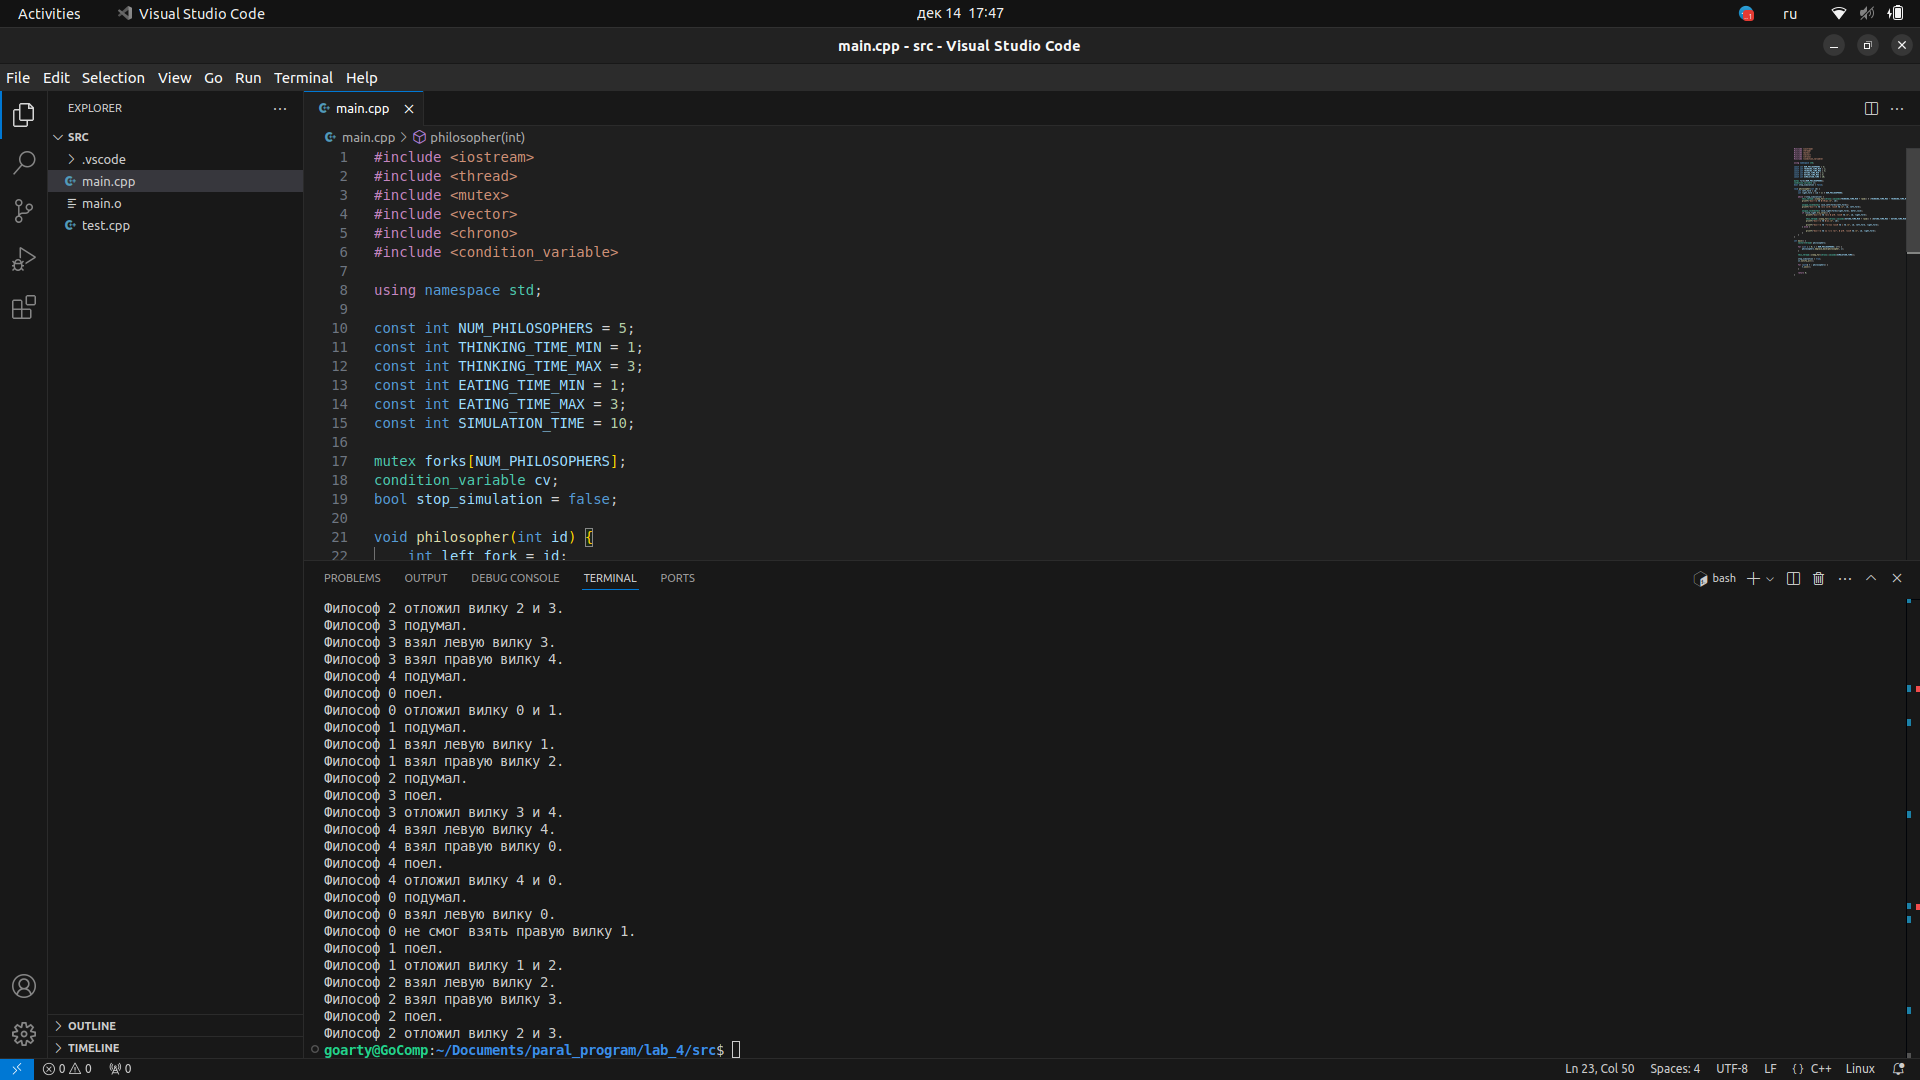
\includegraphics[width=0.8\textwidth]{picture.png}
\label{fig:picture.png}
\end{figure}

\end{document}

